\section{IIQS exclusive parameters}
\label{SECTION:IQS_PARAMS}
In this section we revisit a key parameter of IIQS, the values for $\alpha$ and $\beta$ parameters. As explained previously on Section~\ref{SUBSECTION:IIQS} and in the original work of IIQS~\cite{7416566}, these two values are used during the evaluation of IIQS in order to trigger the execution of a extra partition stage. This extra stage uses a median-of-medians algorithm instead of just relying on the default random pivot selection. The benefit of changing the execution scheme is that it guarantees that the returned median belongs to a position in the central 40 percent of the array.  This extra partition stage has $O(n)$ complexity, hence preserves the original asymptotic bound of the partition algorithm.

\subsection{Understanding median-of-medians usage}
While stated that it does not affect the asymptotic complexity of IQS, it increases its running time by a huge constant factor, as operations performed on BFPRT are not cache friendly for large arrays, specially when implemented in a in-place fashion\footnote{This is because when implemented in-place the idea is not to return the value of the median but rather the index of it. This forces us to move the partial medians generated to a place on which can be cached for next executions and easy controlled. As it is of common knowledge for computer scientists, this position is the beginning of the array.}. 

There is no point on shrinking the \emph{valid area}\footnote{Our central 40\%.} for triggering BFPRT after its evaluation, as there is no guarantee on the resulting distribution of the returned index. Moreover, as BFPRT does not return a median but rather an area on which the median can be found and a partial partitioning of elements~\cite{Blum_Floyd_Pratt_Rivest_Tarjan_1973}, we cannot use this technique as more than a approximate median selection algorithm which shuffles elements along the array.

%% experiment to devise if we can expand the range or we can ignore some bounds.

\begin{figure}[p]
    \centering
    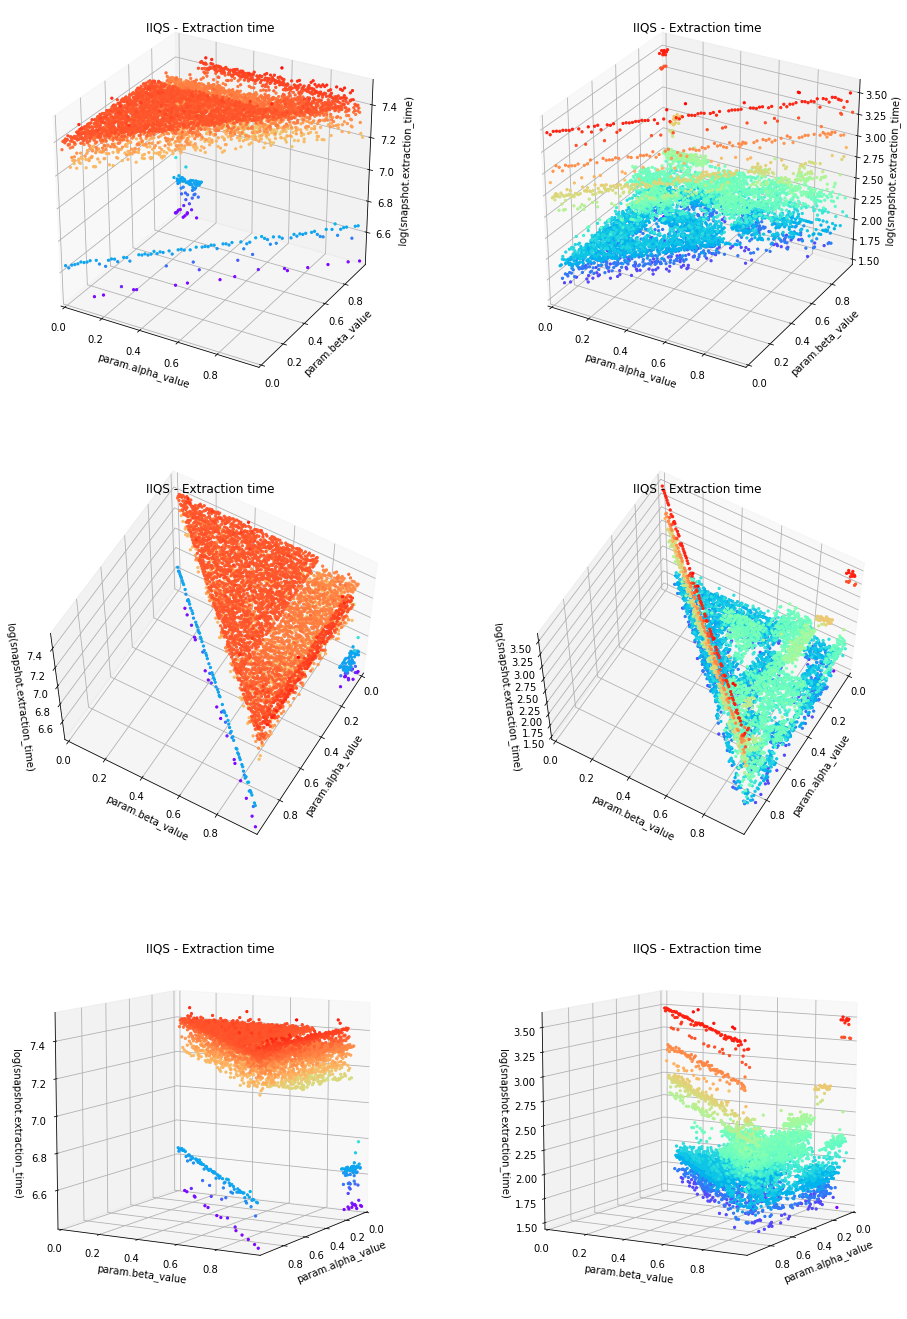
\includegraphics[width=0.8\textwidth]{./fragments/04_experimental_execution/images/04_alphabeta_singleclass.png}
    %\caption{Benchmark for random case. IQS and IIQS executions are shown on the first and second columns respectively.}
    \caption{Benchmark for randomly sorted sequences with $1\times10^6$ unique elements. IIQS executions for the first and second extractions are shown on the first and second column respectively. All extractions using a symlog scale.}
    \label{FIG:05_ALPHABETA_RELATIONSHIP_RANDOM}
\end{figure}

\begin{figure}[p]
    \centering
    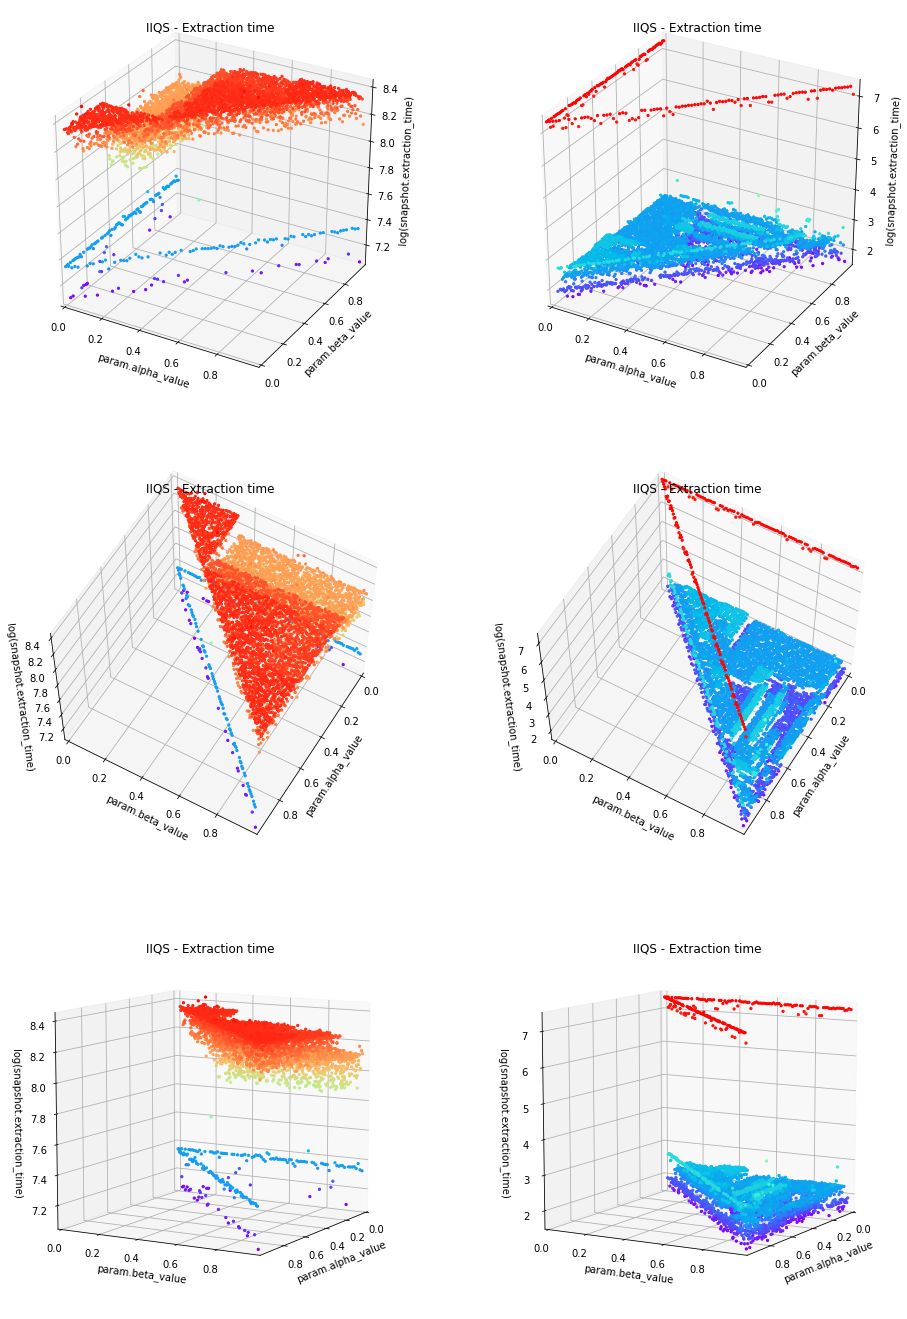
\includegraphics[width=0.8\textwidth]{./fragments/04_experimental_execution/images/04_alphabeta_singleclass_asc.png}
    %\caption{Benchmark for random case. IQS and IIQS executions are shown on the first and second columns respectively.}
    \caption{Benchmark for ascending sequences with $1\times10^6$ unique elements. IIQS executions for the first and second extractions are shown on the first and second column respectively. All extractions using a symlog scale.}
    \label{FIG:05_ALPHABETA_RELATIONSHIP_ASC}
\end{figure}

\begin{figure}[p]
    \centering
    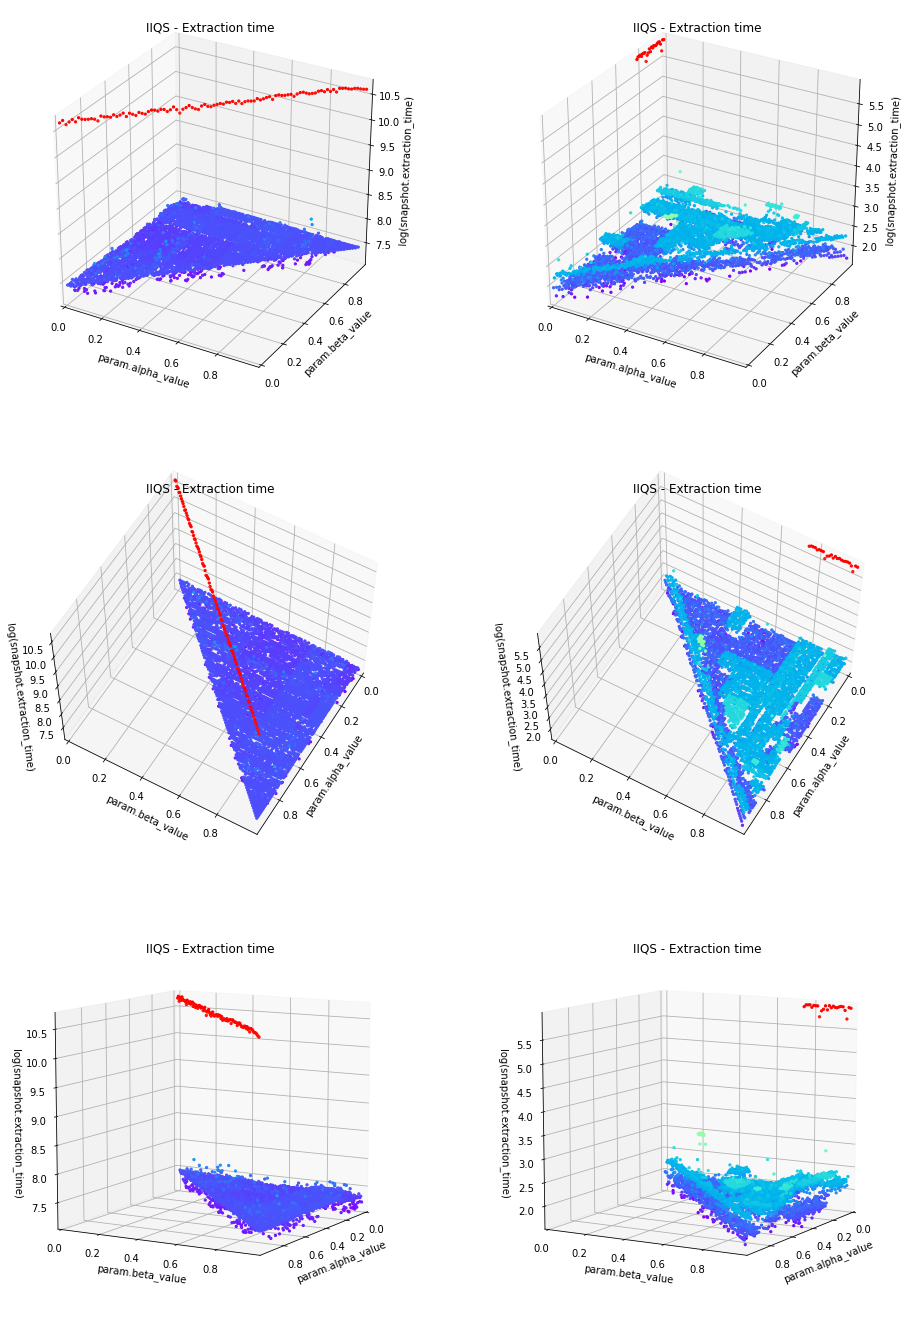
\includegraphics[width=0.8\textwidth]{./fragments/04_experimental_execution/images/04_alphabeta_singleclass_desc.png}
    %\caption{Benchmark for random case. IQS and IIQS executions are shown on the first and second columns respectively.}
    \caption{Benchmark for descending sequences with $1\times10^6$ unique elements. IIQS executions for the first and second extractions are shown on the first and second column respectively. All extractions using a symlog scale.}
    \label{FIG:05_ALPHABETA_RELATIONSHIP_DESC}
\end{figure}


There is a interesting effect resulting of the selection of $\alpha$ and $\beta$ parameters. By just examining the first and second extractions we can appreciate that if we tight the bounds to a point that median-of-medians is executed each time, for all instances we get that the first extraction is accelerated by a huge factor but that comes at a cost of the second extraction being three orders of magnitude larger than the average execution. There is a ton of room for different behaviors on this implementation as we can check when comparing the execution for each dataset, the regions that seems to be best performing for one are the worst for another case.

But something that it is common is that closing the bound too tight affects negatively the running time as well as to completely ignore the value of $\alpha$ parameter, at least when fixing all constraints to force a worst-case running time. That is, by fixing the pivot-bias to select the leftmost element. By extension, this applies to the other possible values for the pivot bias. 


\subsection{Relaxation of $\alpha$ and $\beta$ constraints}

As stated by BFPRT definition, as the pivot returned belongs to the middle 40 percent of the array, there is no need to run IIQS if our pivot already belongs to this segment. But yet there is no insight on if relaxing the constraints for IIQS $\alpha$ and $\beta$ parameters does have any impact on its running time. As seen on figures there are some configurations which favour certain scenarios. On this first analysis presented on Figures~\ref{FIG:05_ALPHABETA_BENCHMARK_RANDOM},~\ref{FIG:05_ALPHABETA_BENCHMARK_ASC}~and~\ref{FIG:05_ALPHABETA_BENCHMARK_DESC} we can appreciate that futher relaxation of $\alpha$ and $\beta$ parameters contribute to noticeable improvements over running time without affecting in most cases the quality of the stack in certain cases. Furthermore, as there is no combination which gets closer to an all-cases resistant implementation, we conclude that relaxation of such parameters outside of their guaranteed bounds does not contribute to the development of a general usage version of IIQS.

\begin{figure}[p]
    \centering
    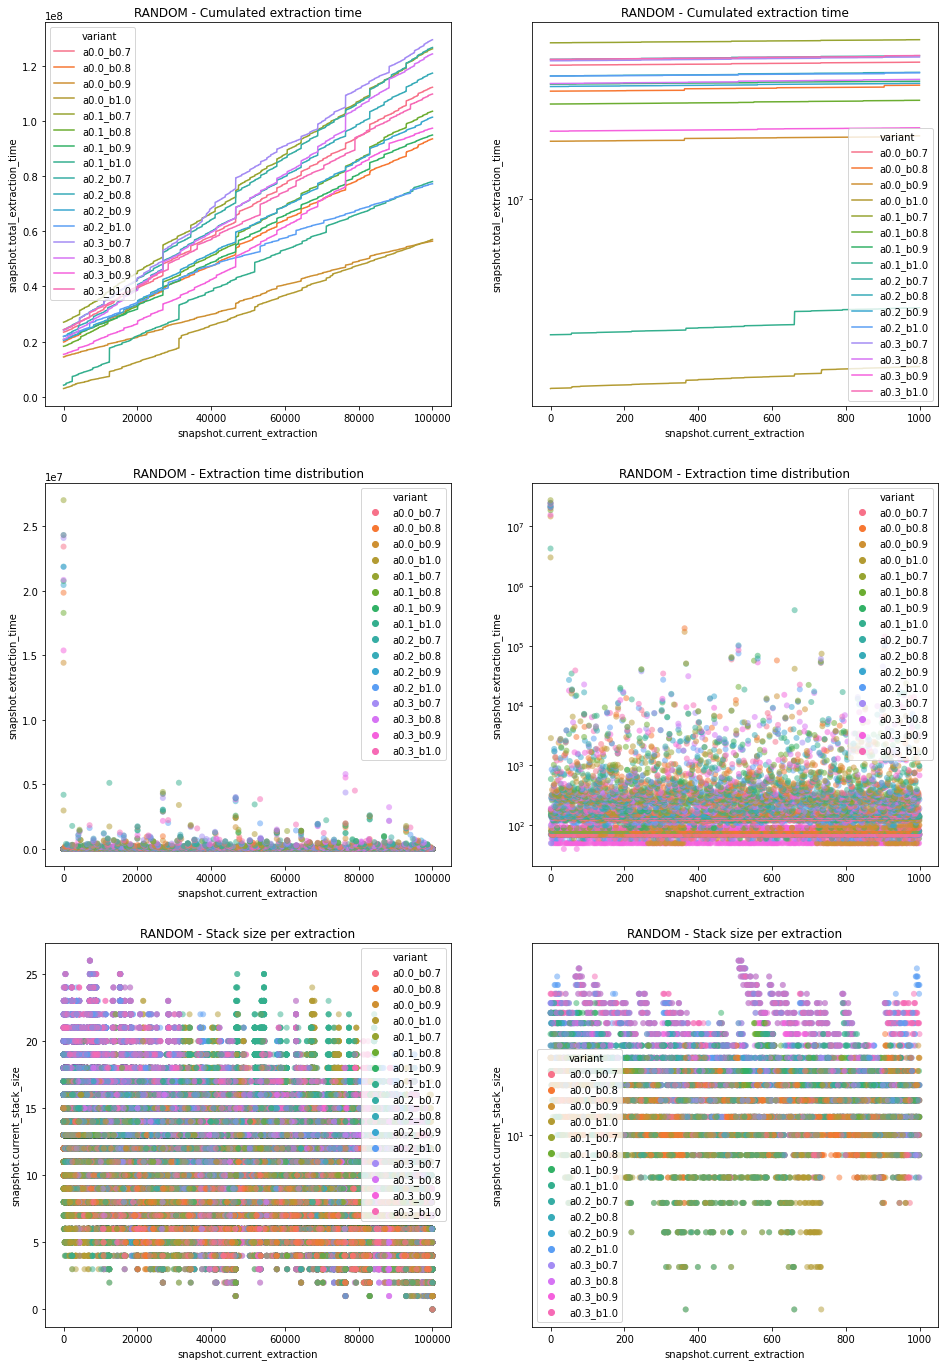
\includegraphics[width=0.79\textwidth]{./fragments/04_experimental_execution/images/04_alphabeta_detail_random.png}
    %\caption{Benchmark for random case. IQS and IIQS executions are shown on the first and second columns respectively.}
    \caption{Benchmark for randomly sorted sequences with $1\times10^5$ unique elements for IIQS. This benchmark covers rough combinations of relaxations for BFPRT parameters. First column represents all extractions using a linear scale. Second column depicts a logarithmic scale and shows the first $1\times10^3$ extractions. }
    \label{FIG:05_ALPHABETA_BENCHMARK_RANDOM}
\end{figure}

\begin{figure}[p]
    \centering
    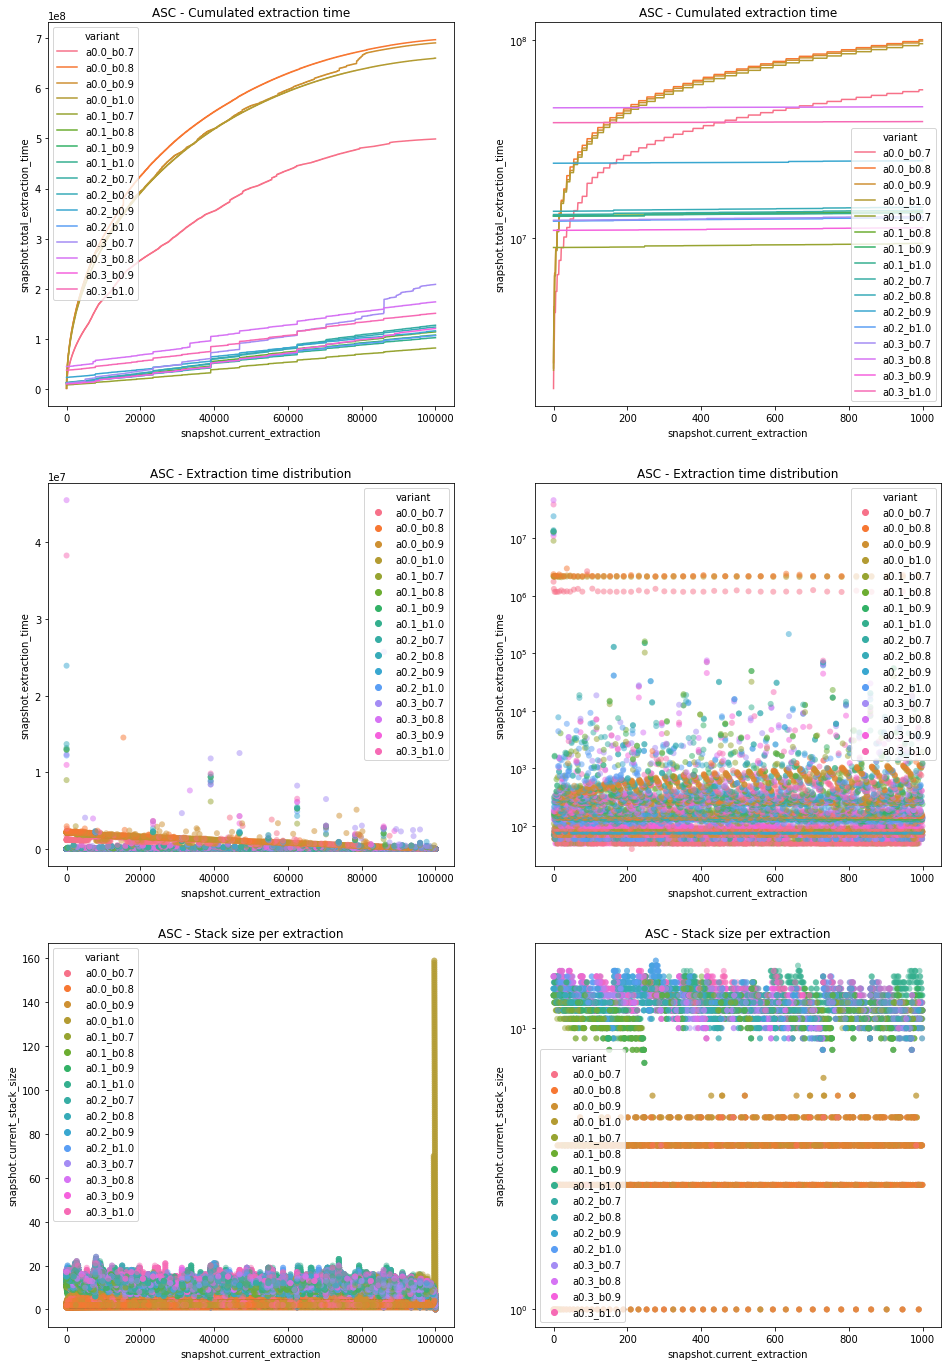
\includegraphics[width=0.79\textwidth]{./fragments/04_experimental_execution/images/04_alphabeta_detail_increasing.png}
    %\caption{Benchmark for random case. IQS and IIQS executions are shown on the first and second columns respectively.}
    \caption{Benchmark for increasing sequences with $1\times10^5$ unique elements for IIQS. This benchmark covers rough combinations of relaxations for BFPRT parameters. First column represents all extractions using a linear scale. Second column depicts a logarithmic scale and shows the first $1\times10^3$ extractions. }
    \label{FIG:05_ALPHABETA_BENCHMARK_ASC}
\end{figure}

\begin{figure}[p]
    \centering
    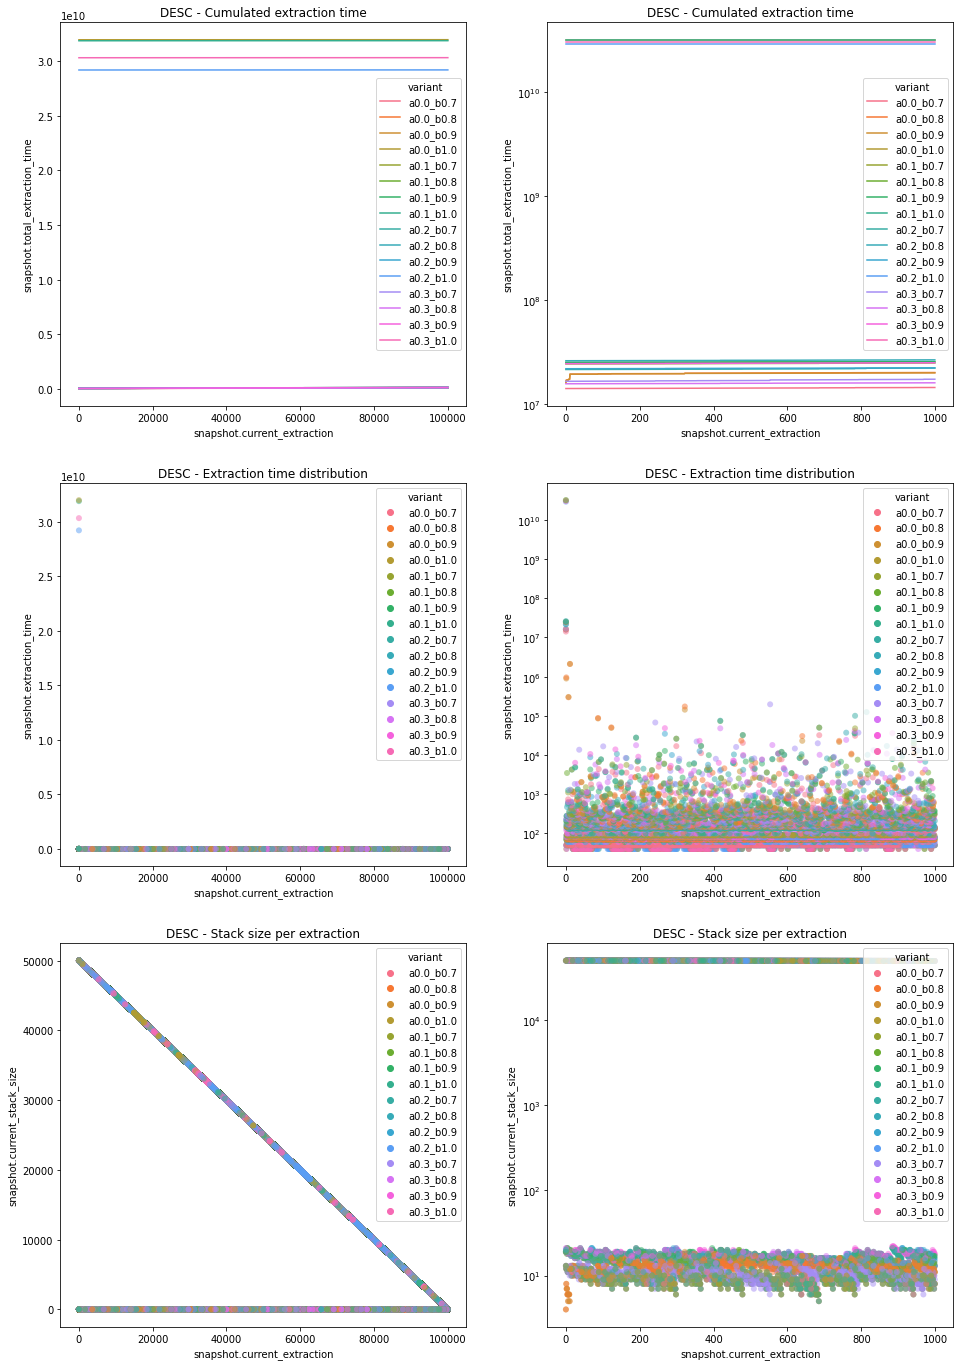
\includegraphics[width=0.79\textwidth]{./fragments/04_experimental_execution/images/04_alphabeta_detail_decreasing.png}
    %\caption{Benchmark for random case. IQS and IIQS executions are shown on the first and second columns respectively.}
    \caption{Benchmark for decreasing sequences with $1\times10^5$ unique elements for IIQS. This benchmark covers rough combinations of relaxations for BFPRT parameters. First column represents all extractions using a linear scale. Second column depicts a logarithmic scale and shows the first $1\times10^3$ extractions. }
    \label{FIG:05_ALPHABETA_BENCHMARK_DESC}
\end{figure}


\subsection{Tightening $\alpha$ and $\beta$ constraints for unique elements}

As for independent tuning of $\alpha$ beta shown in Figures~\ref{FIG:05_ALPHABETA_BENCHMARK_RANDOM_LEFT},~\ref{FIG:05_ALPHABETA_BENCHMARK_ASC_LEFT}, and~\ref{FIG:05_ALPHABETA_BENCHMARK_DESC_LEFT} and $\beta$ parameter shown in Figures~\ref{FIG:05_ALPHABETA_BENCHMARK_RANDOM_RIGHT},~\ref{FIG:05_ALPHABETA_BENCHMARK_ASC_RIGHT}, and~\ref{FIG:05_ALPHABETA_BENCHMARK_DESC_RIGHT}, there is no relaxation available outside of the expected bounds for BFPRT unless we are expecting to optimize the execution for certain distributions.

A total opposite of the previous case, as it does seem that tightening BFPRT parameters does not contribute at lowering our current upper bound nor to changing it at all. But different to our initial expectations, it does seem that for certain combinations we obtain in average a better performance on all cases for non repeated elements in the sequence. This is the case of $\alpha=0.5$ and $\beta=0.65$, which appears as the best performant combination of parameters on Figures~\ref{FIG:05_ALPHABETA_BENCHMARK_RANDOM_INNER},~\ref{FIG:05_ALPHABETA_BENCHMARK_ASC_INNER}, and~\ref{FIG:05_ALPHABETA_BENCHMARK_DESC_INNER}. 


\begin{figure}[p]
    \centering
    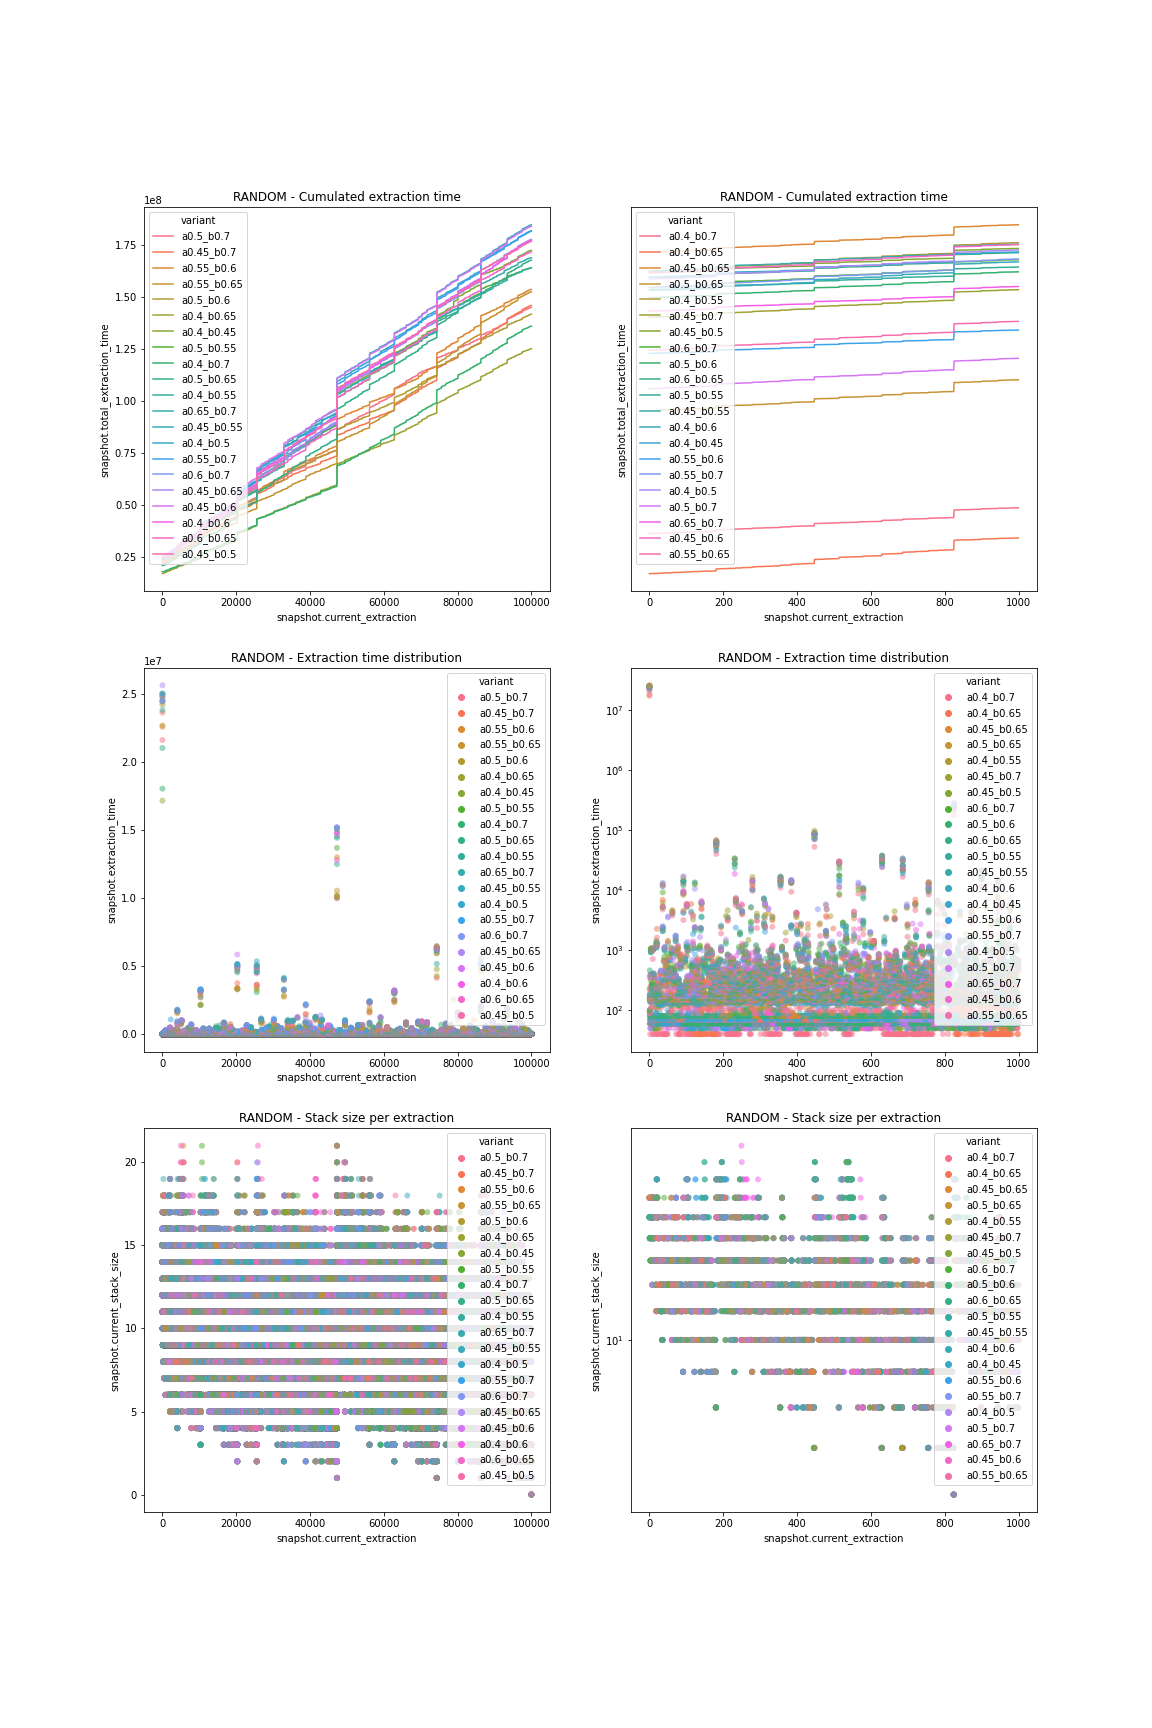
\includegraphics[width=0.79\textwidth]{./fragments/04_experimental_execution/images/04_alphabeta_detail_random_inner.png}
    %\caption{Benchmark for random case. IQS and IIQS executions are shown on the first and second columns respectively.}
    \caption{Benchmark for randomly sorted sequences with $1\times10^5$ unique elements for IIQS. This benchmark only covers the expected return section of BFPRT. First column represents all extractions using a linear scale. Second column depicts a logarithmic scale and shows the first $1\times10^3$ extractions. }
    \label{FIG:05_ALPHABETA_BENCHMARK_RANDOM_INNER}
\end{figure}

\begin{figure}[p]
    \centering
    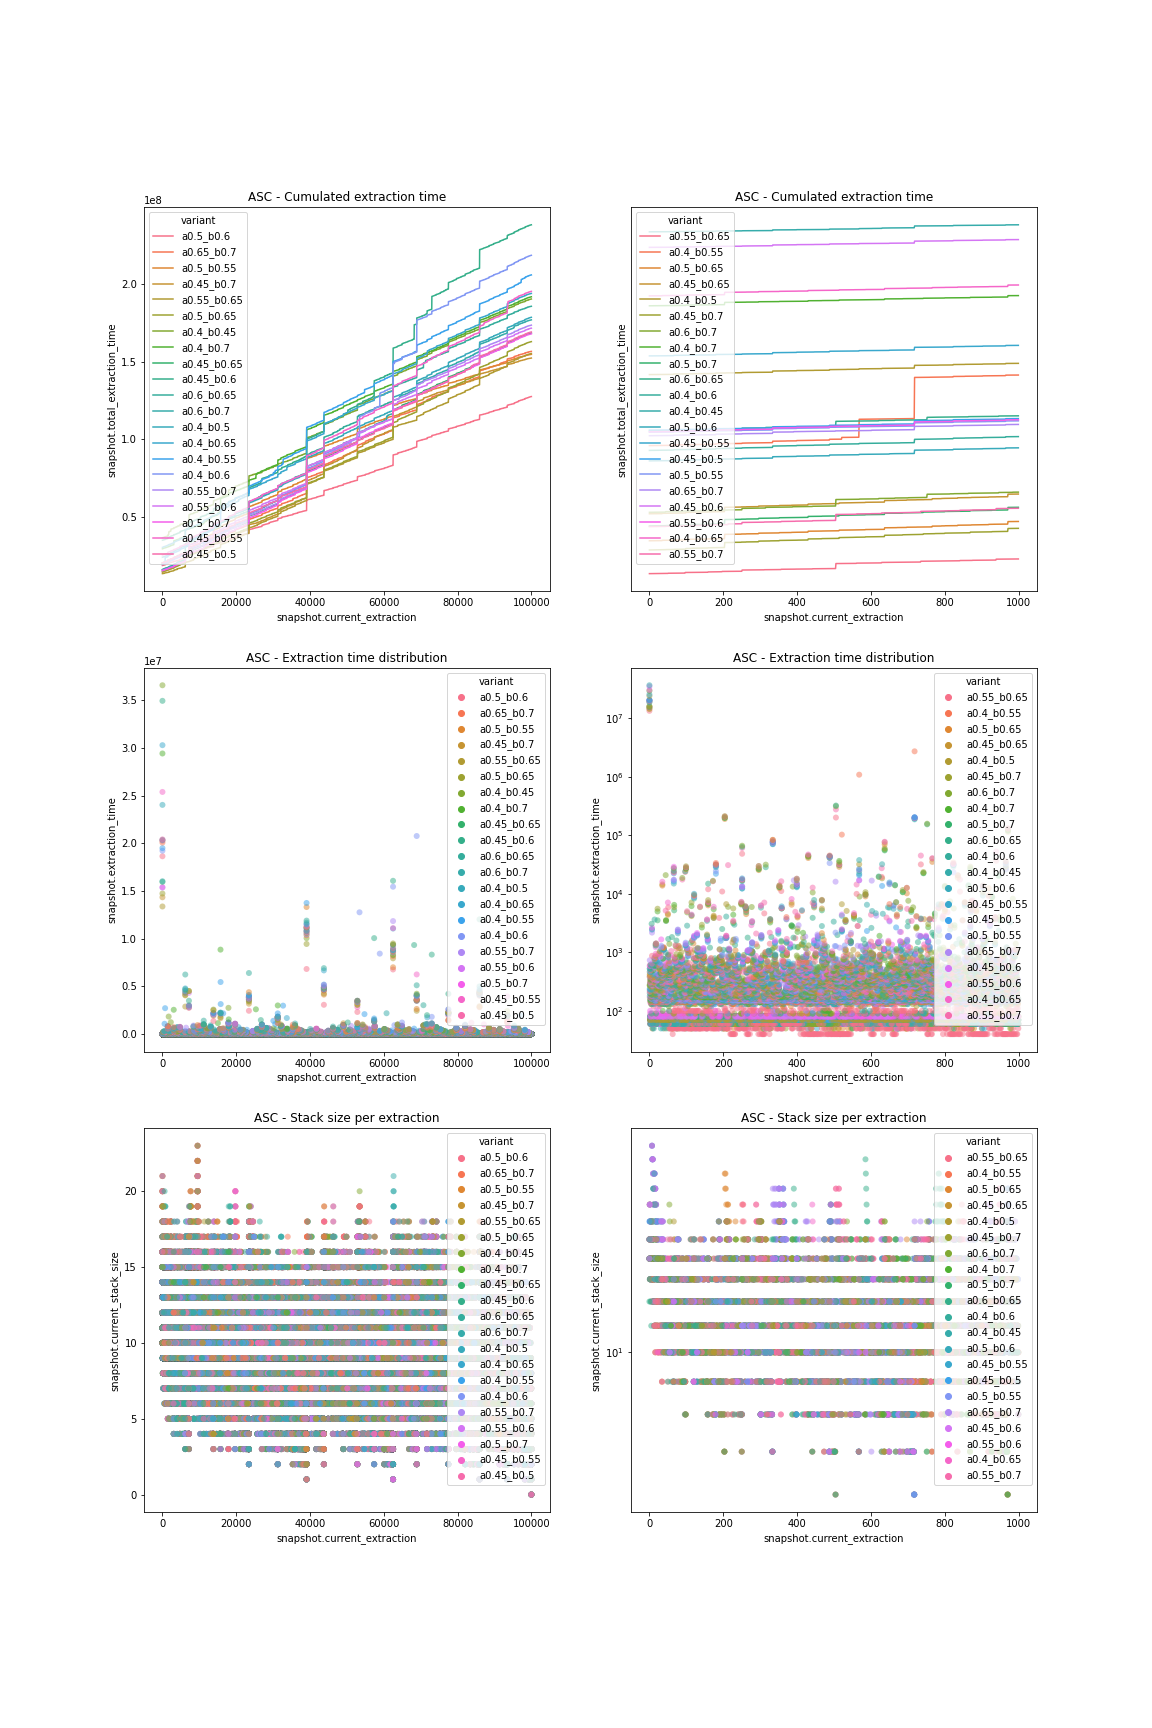
\includegraphics[width=0.79\textwidth]{./fragments/04_experimental_execution/images/04_alphabeta_detail_increasing_inner.png}
    %\caption{Benchmark for random case. IQS and IIQS executions are shown on the first and second columns respectively.}
    \caption{Benchmark for increasing sequences with $1\times10^5$ unique elements for IIQS. This benchmark only covers the expected return section of BFPRT. First column represents all extractions using a linear scale. Second column depicts a logarithmic scale and shows the first $1\times10^3$ extractions. }
    \label{FIG:05_ALPHABETA_BENCHMARK_ASC_INNER}
\end{figure}

\begin{figure}[p]
    \centering
    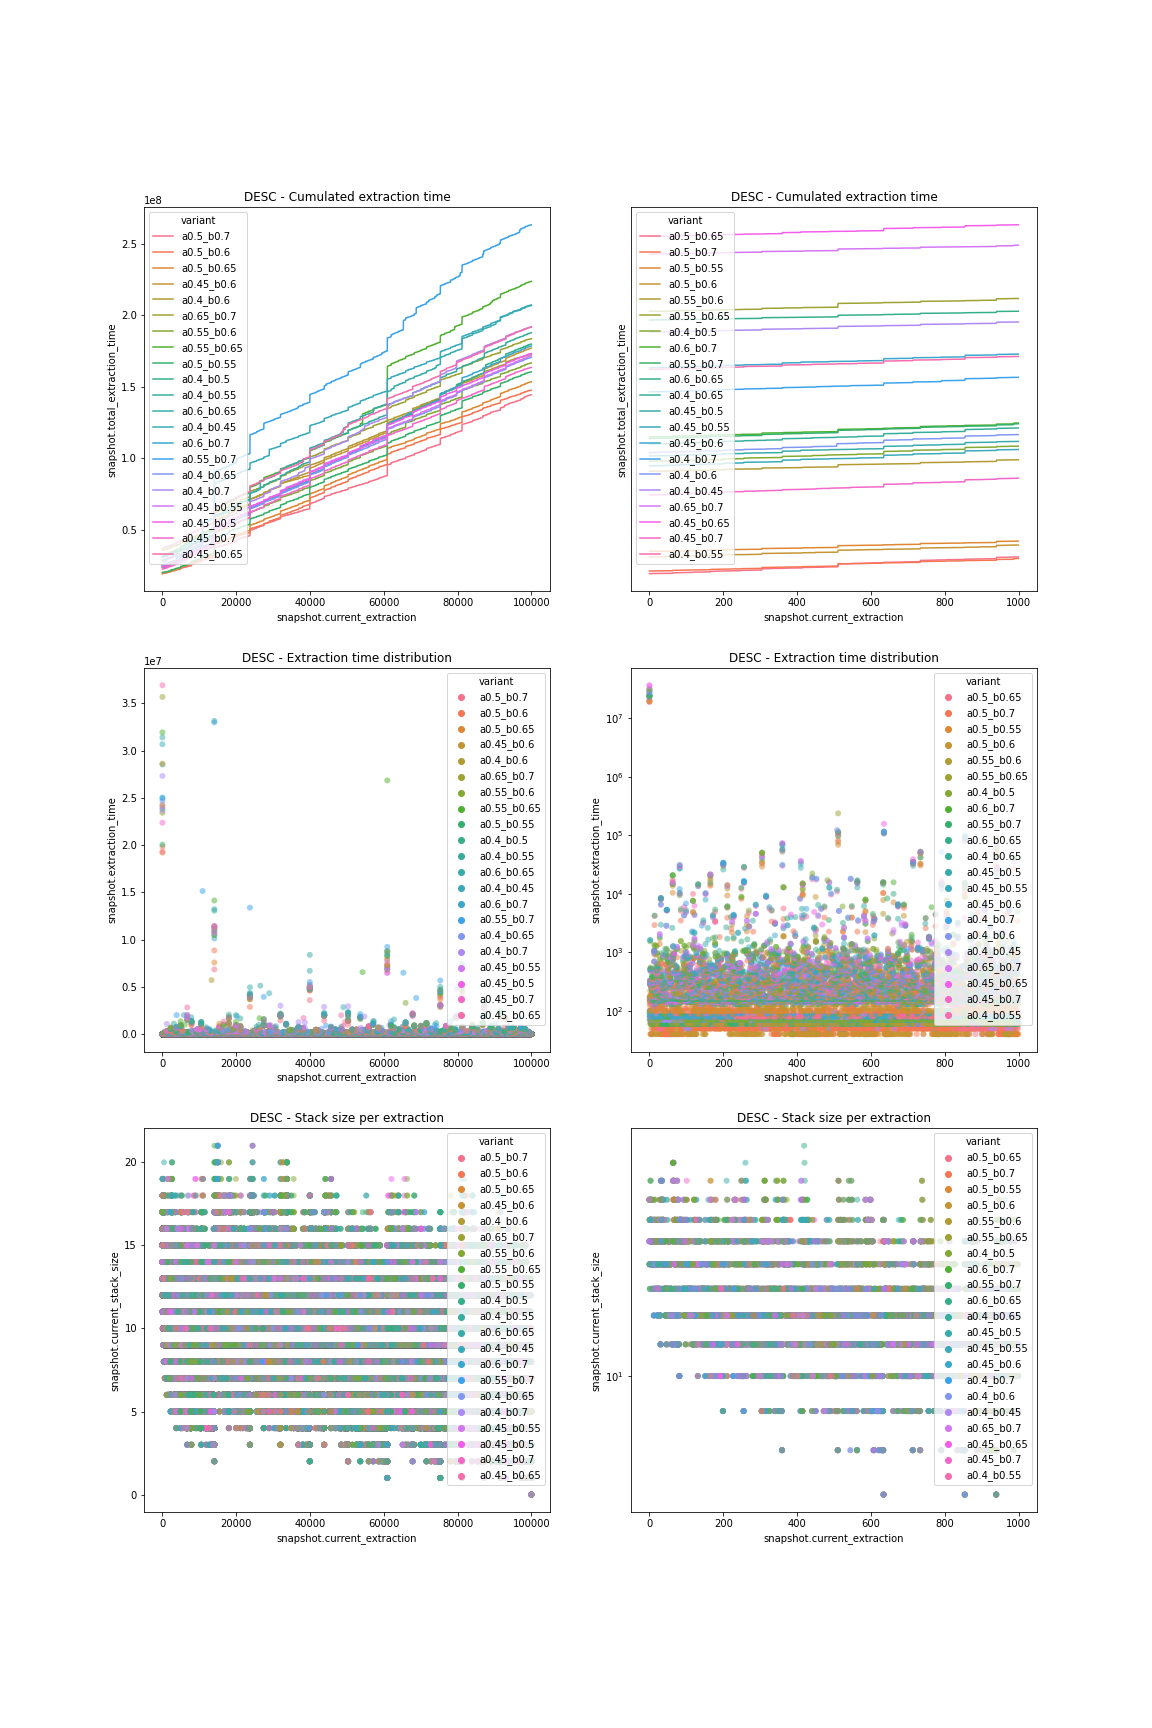
\includegraphics[width=0.79\textwidth]{./fragments/04_experimental_execution/images/04_alphabeta_detail_decreasing_inner.png}
    %\caption{Benchmark for random case. IQS and IIQS executions are shown on the first and second columns respectively.}
    \caption{Benchmark for decreasing sequences with $1\times10^5$ unique elements for IIQS. This benchmark only covers the expected return section of BFPRT. First column represents all extractions using a linear scale. Second column depicts a logarithmic scale and shows the first $1\times10^3$ extractions. }
    \label{FIG:05_ALPHABETA_BENCHMARK_DESC_INNER}
\end{figure}

\begin{figure}[p]
    \centering
    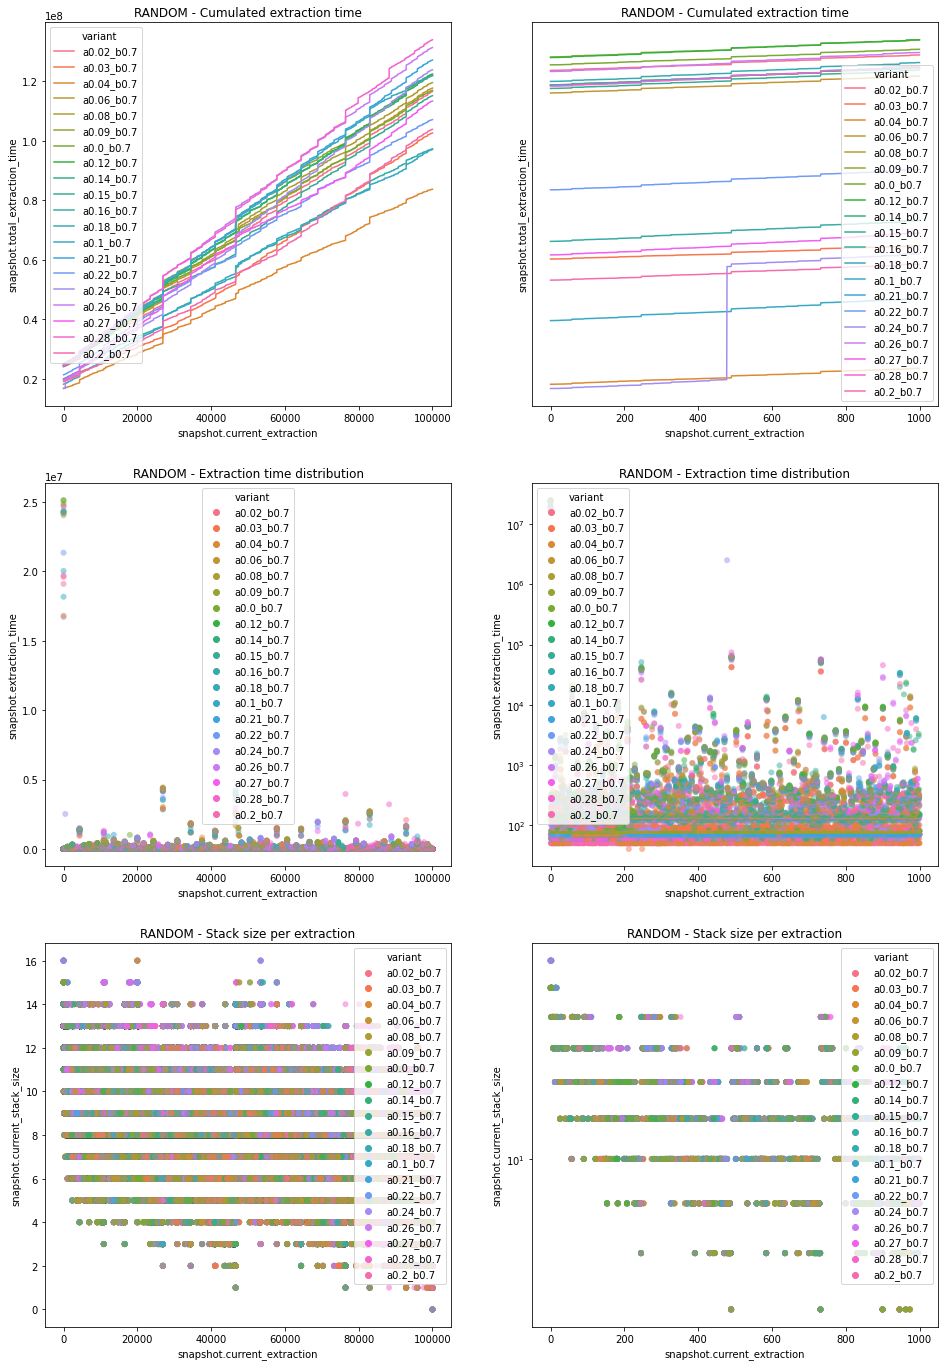
\includegraphics[width=0.79\textwidth]{./fragments/04_experimental_execution/images/04_alphabeta_detail_random_left.png}
    %\caption{Benchmark for random case. IQS and IIQS executions are shown on the first and second columns respectively.}
    \caption{Benchmark for randomly sorted sequences with $1\times10^5$ unique elements for IIQS. This covers a detailed view of relaxations for $\alpha$ parameter while fixing $\beta=0.7$. First column represents all extractions using a linear scale. Second column depicts a logarithmic scale and shows the first $1\times10^3$ extractions. }
    \label{FIG:05_ALPHABETA_BENCHMARK_RANDOM_LEFT}
\end{figure}

\begin{figure}[p]
    \centering
    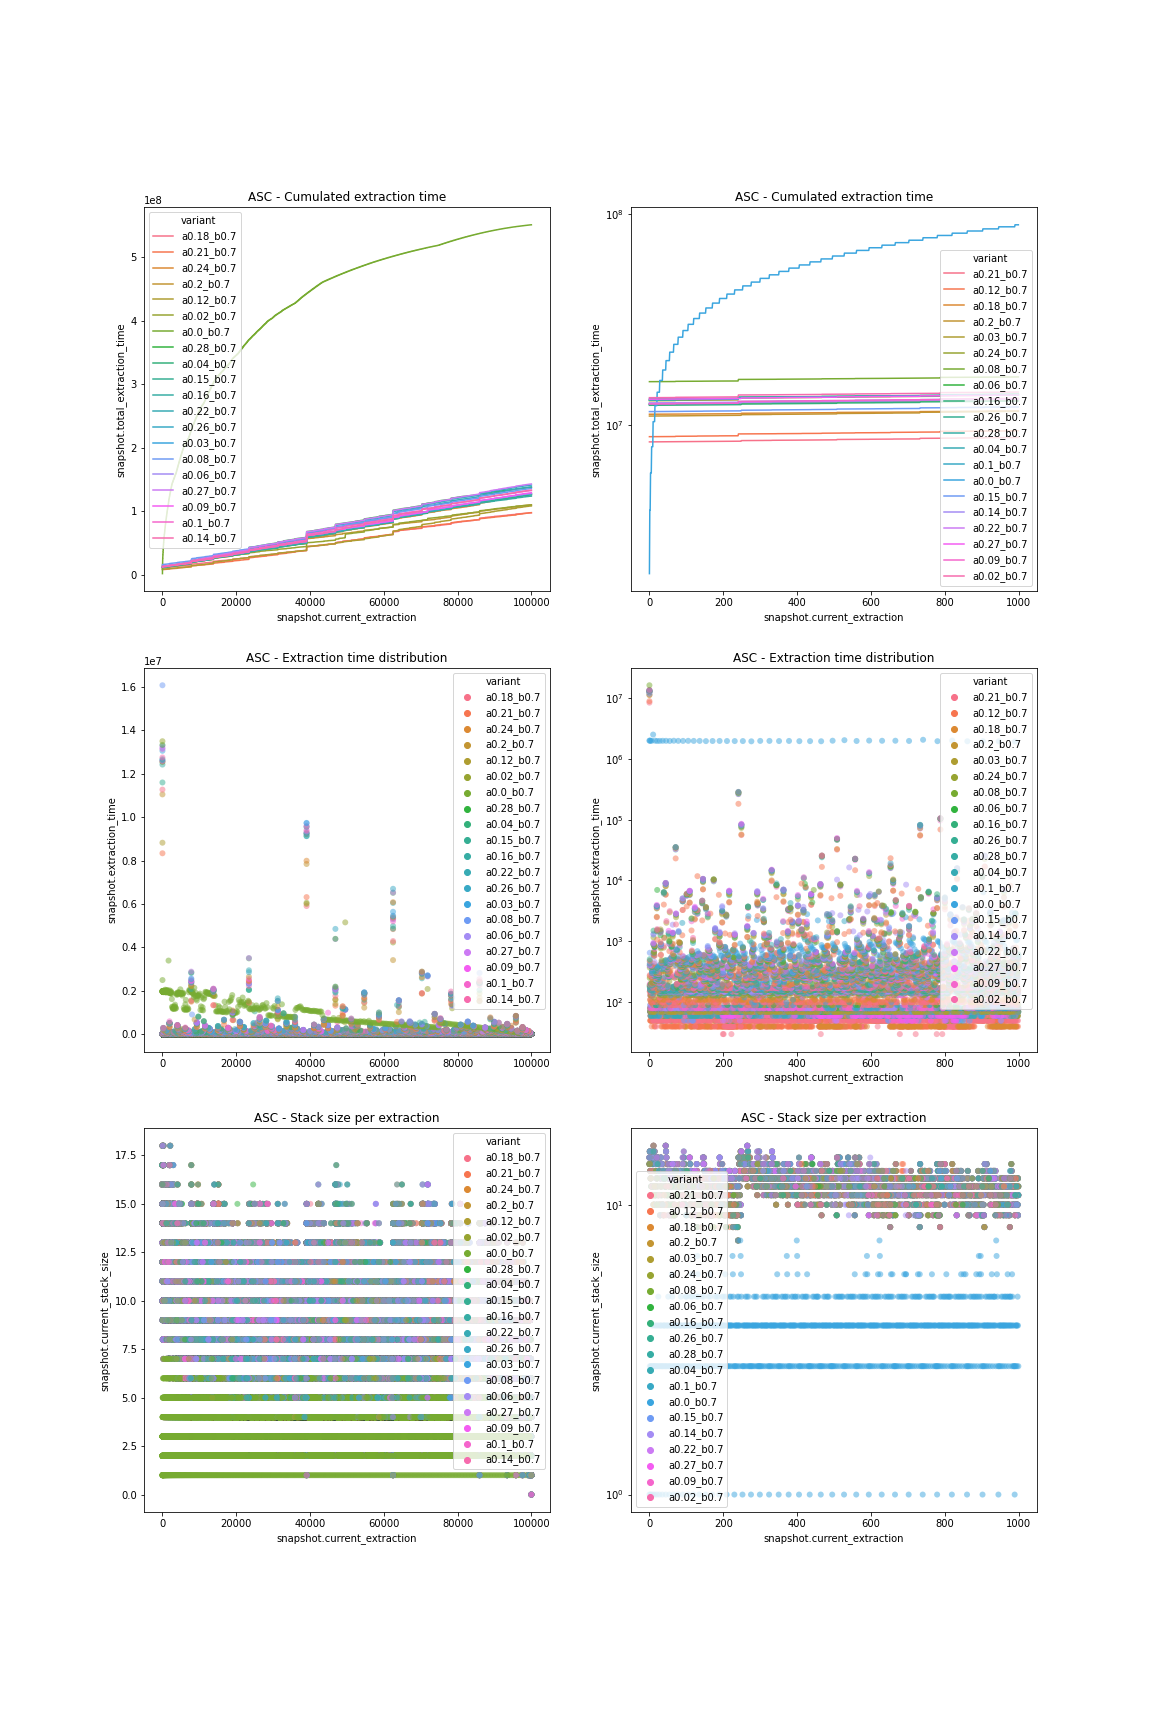
\includegraphics[width=0.79\textwidth]{./fragments/04_experimental_execution/images/04_alphabeta_detail_increasing_left.png}
    %\caption{Benchmark for random case. IQS and IIQS executions are shown on the first and second columns respectively.}
    \caption{Benchmark for increasing sequences with $1\times10^5$ unique elements for IIQS. This covers a detailed view of relaxations for $\alpha$ parameter while fixing $\beta=0.7$. First column represents all extractions using a linear scale. Second column depicts a logarithmic scale and shows the first $1\times10^3$ extractions. }
    \label{FIG:05_ALPHABETA_BENCHMARK_ASC_LEFT}
\end{figure}

\begin{figure}[p]
    \centering
    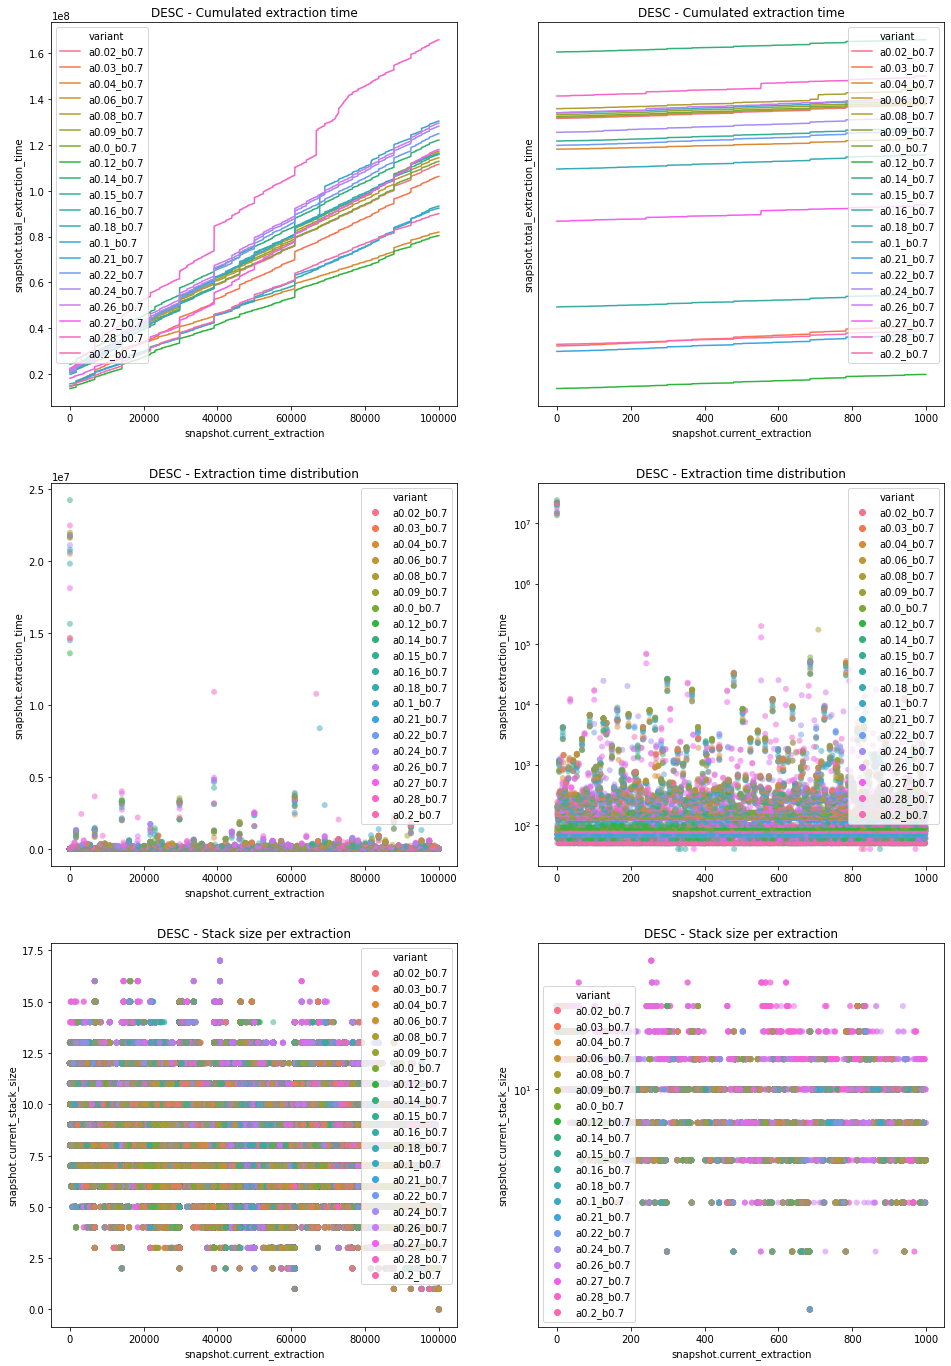
\includegraphics[width=0.79\textwidth]{./fragments/04_experimental_execution/images/04_alphabeta_detail_decreasing_left.png}
    %\caption{Benchmark for random case. IQS and IIQS executions are shown on the first and second columns respectively.}
    \caption{Benchmark for decreasing sequences with $1\times10^5$ unique elements for IIQS. This covers a detailed view of relaxations for $\alpha$ parameter while fixing $\beta=0.7$. First column represents all extractions using a linear scale. Second column depicts a logarithmic scale and shows the first $1\times10^3$ extractions. }
    \label{FIG:05_ALPHABETA_BENCHMARK_DESC_LEFT}
\end{figure}

\begin{figure}[p]
    \centering
    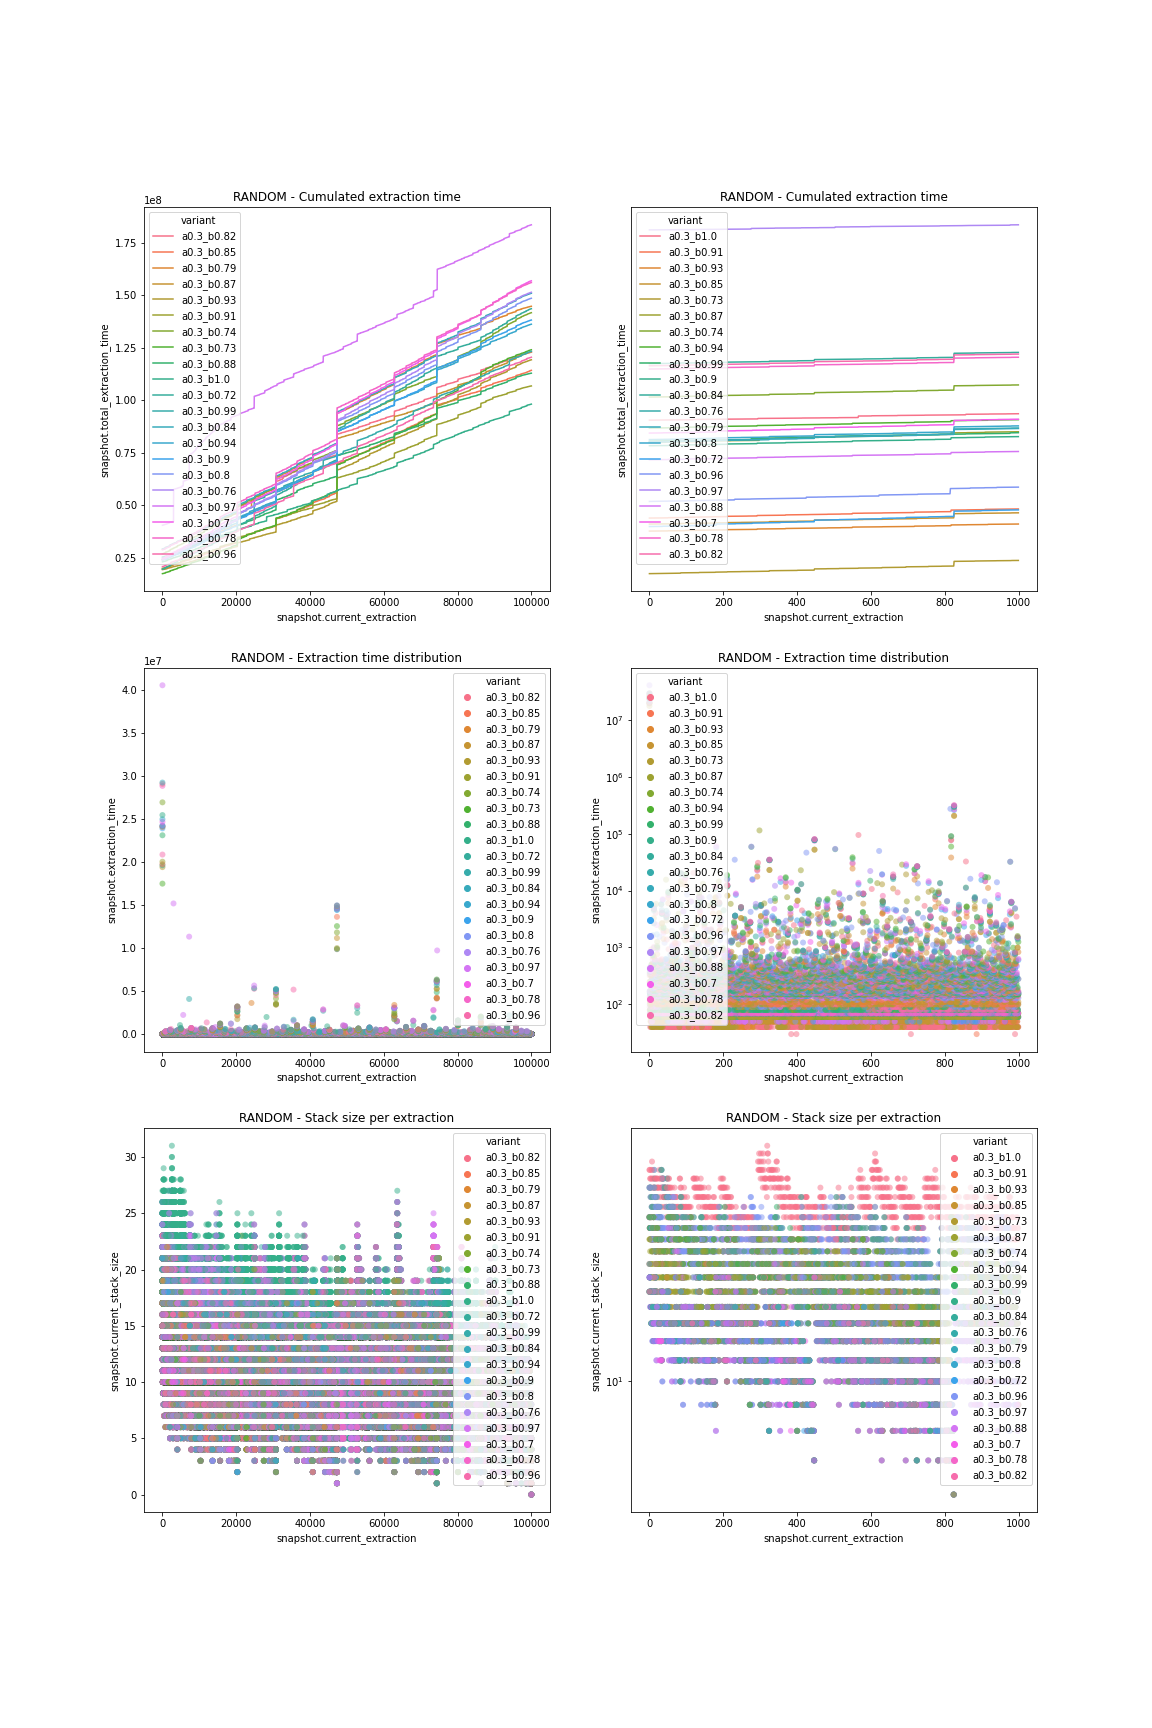
\includegraphics[width=0.79\textwidth]{./fragments/04_experimental_execution/images/04_alphabeta_detail_random_right.png}
    %\caption{Benchmark for random case. IQS and IIQS executions are shown on the first and second columns respectively.}
    \caption{Benchmark for randomly sorted sequences with $1\times10^5$ unique elements for IIQS. This covers a detailed view of relaxations for $\beta$ parameter while fixing $\alpha=0.3$.  First column represents all extractions using a linear scale. Second column depicts a logarithmic scale and shows the first $1\times10^3$ extractions. }
    \label{FIG:05_ALPHABETA_BENCHMARK_RANDOM_RIGHT}
\end{figure}

\begin{figure}[p]
    \centering
    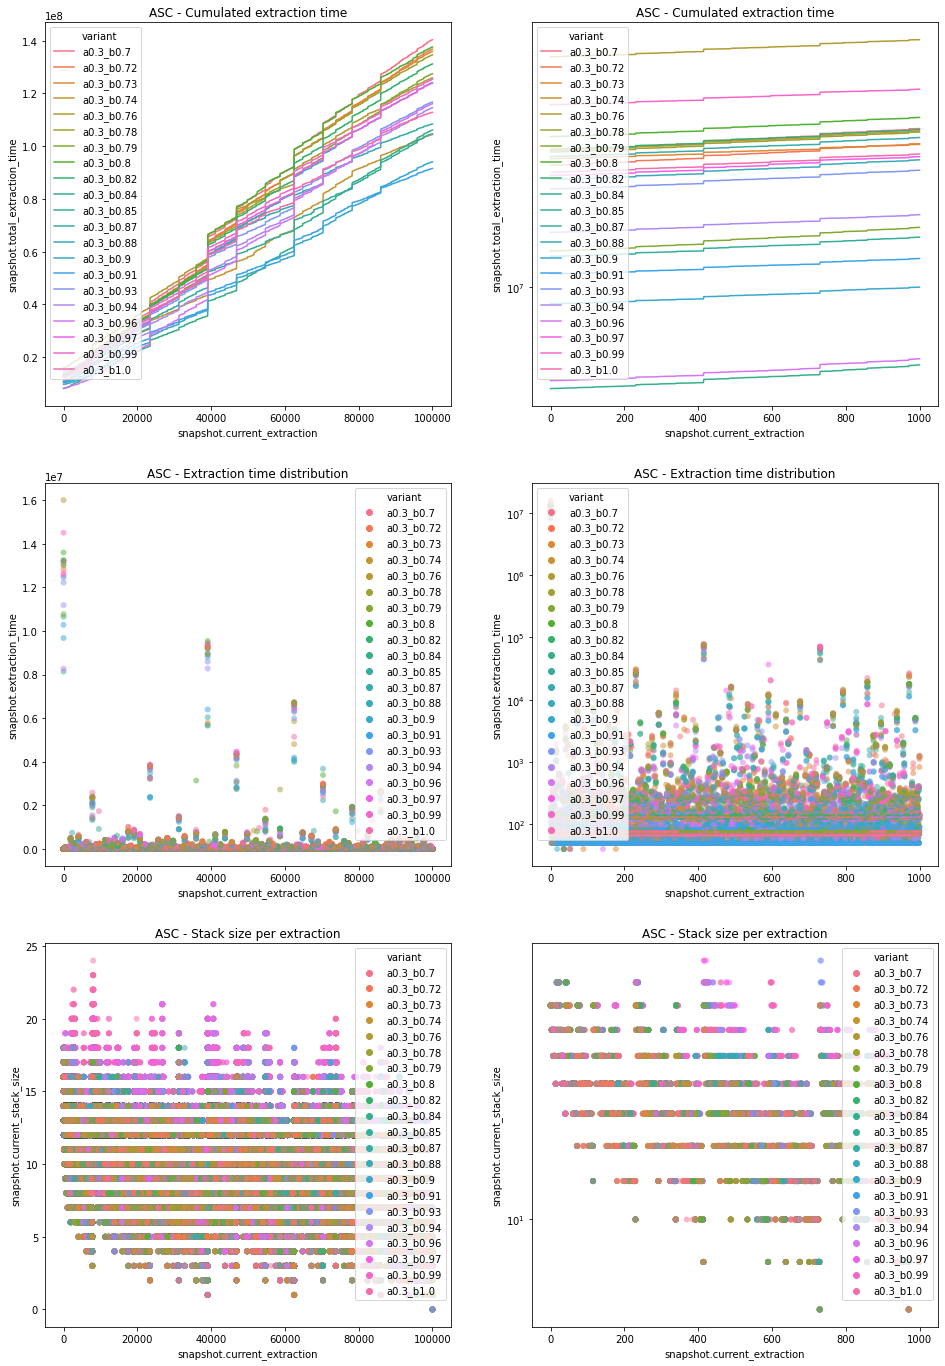
\includegraphics[width=0.79\textwidth]{./fragments/04_experimental_execution/images/04_alphabeta_detail_increasing_right.png}
    %\caption{Benchmark for random case. IQS and IIQS executions are shown on the first and second columns respectively.}
    \caption{Benchmark for increasing sequences with $1\times10^5$ unique elements for IIQS. This covers a detailed view of relaxations for $\beta$ parameter while fixing $\alpha=0.3$.  First column represents all extractions using a linear scale. Second column depicts a logarithmic scale and shows the first $1\times10^3$ extractions. }
    \label{FIG:05_ALPHABETA_BENCHMARK_ASC_RIGHT}
\end{figure}

\begin{figure}[p]
    \centering
    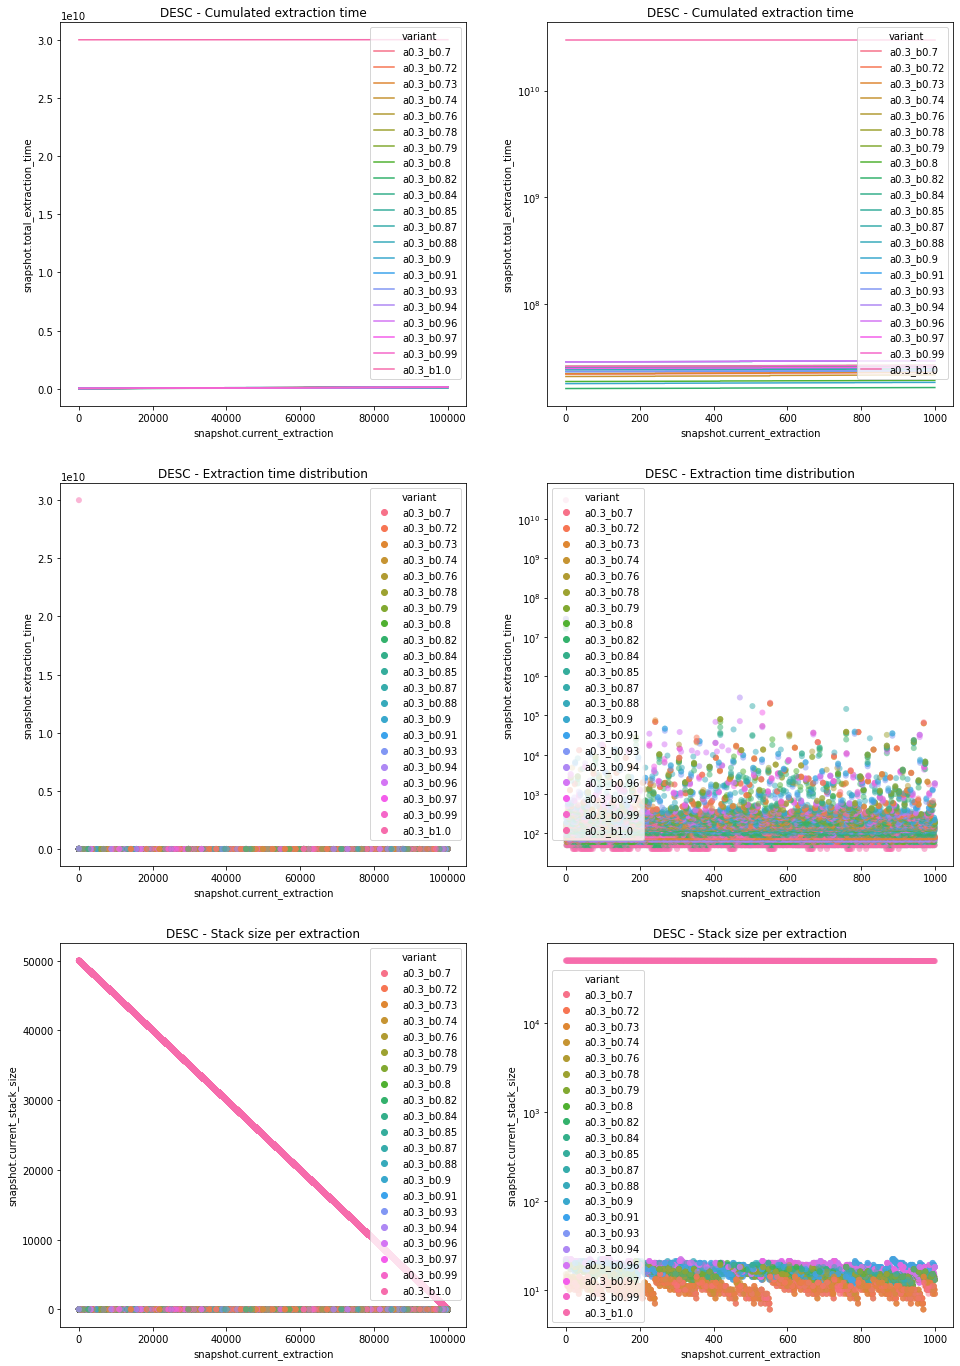
\includegraphics[width=0.79\textwidth]{./fragments/04_experimental_execution/images/04_alphabeta_detail_decreasing_right.png}
    %\caption{Benchmark for random case. IQS and IIQS executions are shown on the first and second columns respectively.}
    \caption{Benchmark for decreasing sequences with $1\times10^5$ unique elements for IIQS. This covers a detailed view of relaxations for $\beta$ parameter while fixing $\alpha=0.3$.  First column represents all extractions using a linear scale. Second column depicts a logarithmic scale and shows the first $1\times10^3$ extractions. }
    \label{FIG:05_ALPHABETA_BENCHMARK_DESC_RIGHT}
\end{figure}

\subsection{Effect of repeated elements in the sequence}

Further testing against the more aggressive situation for IIQS reveals that there are two cases when dealing with repeated elements on IIQS. When there is only one class across the entire sequence a performance boost for all extractions is only achieved by continuously executing IIQS on all iterations. In other cases, the performance is degraded by at least two orders of magnitude. More interesting, for all cases on which BFPRT were executed, the stack size remained stable with a solid %TODO: finish this

\begin{figure}[p]
    \centering
    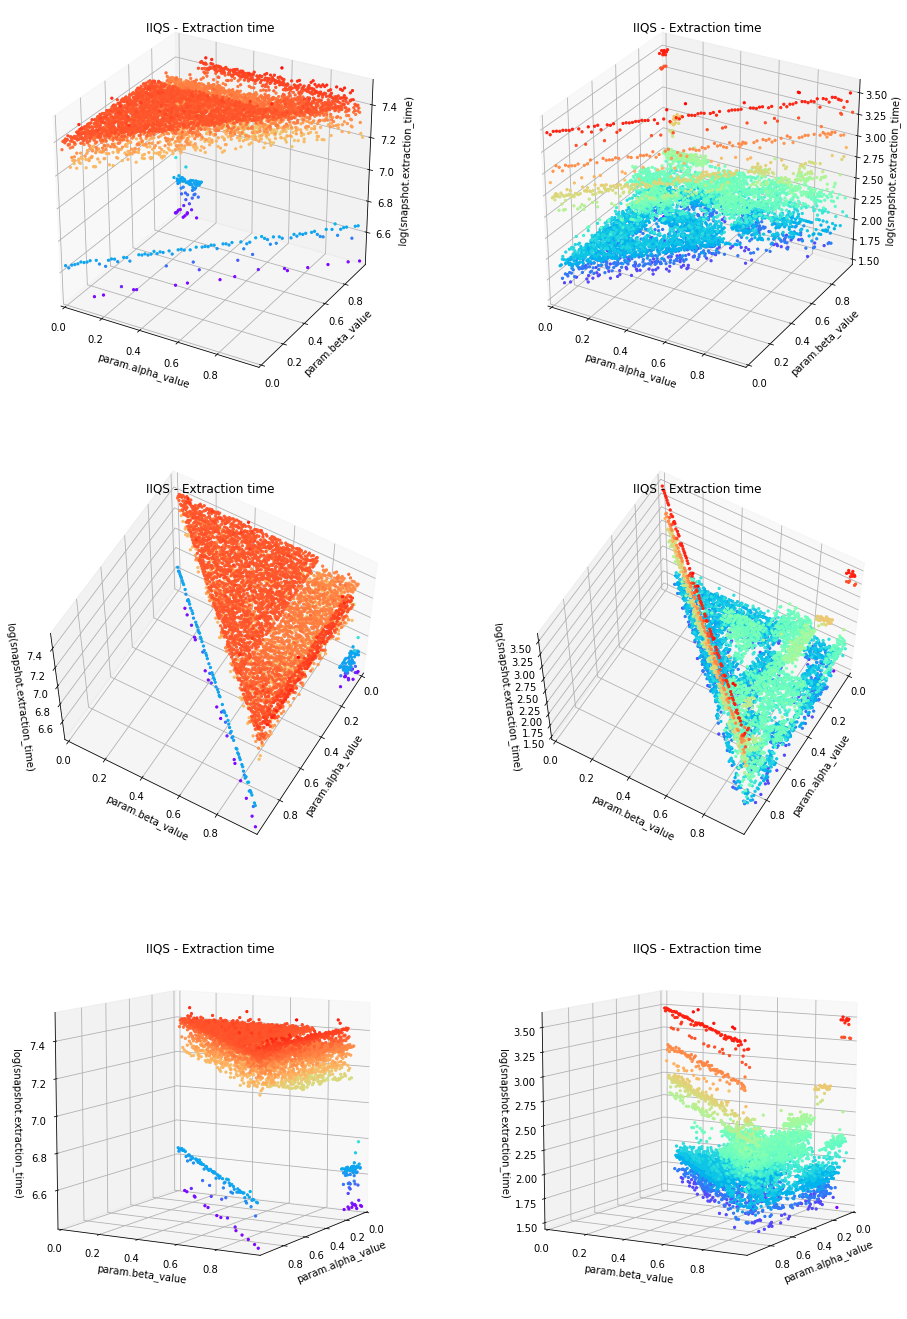
\includegraphics[width=0.8\textwidth]{./fragments/04_experimental_execution/images/04_alphabeta_singleclass.png}
    %\caption{Benchmark for random case. IQS and IIQS executions are shown on the first and second columns respectively.}
    \caption{Benchmark for sequences with $1\times10^4$ repeated elements as a single class. IIQS executions for the first and second extractions are shown on the first and second column respectively. All extractions using a symlog scale.}
    \label{FIG:05_ALPHABETA_RELATIONSHIP_SINGLECLASS}
\end{figure}



\begin{figure}[p]
    \centering
    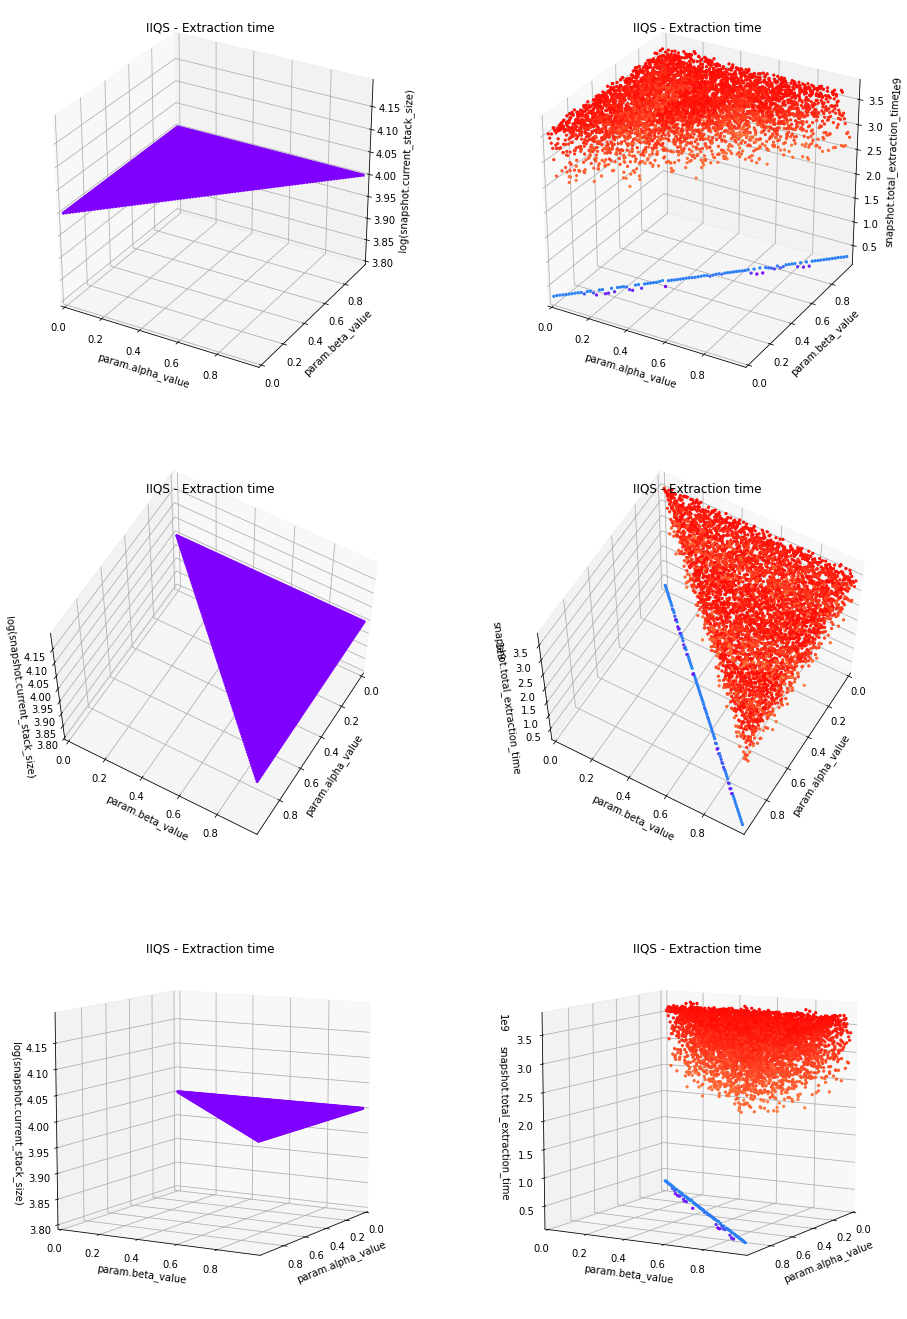
\includegraphics[width=0.8\textwidth]{./fragments/04_experimental_execution/images/04_alphabeta_singleclass_stack.png}
    %\caption{Benchmark for random case. IQS and IIQS executions are shown on the first and second columns respectively.}
    \caption{Benchmark for sequences with $1\times10^4$ repeated elements as a single class. IIQS stack size for the first and second extractions are shown on the first and second column respectively. All extractions using a symlog scale.}
    \label{FIG:05_ALPHABETA_RELATIONSHIP_SINGLECLASS_STACK}
\end{figure}

As by examining the results depicted in Figures and~\ref{FIG:05_ALPHABETA_RELATIONSHIP_SINGLECLASS_STACK}, we can conclude that changing IIQS parameters does not affect the performance when dealing with repeated elements, as the bias for returning a position on the BFPRT result as pivot is the one directly impacting the performance and not the bounds for BFPRT execution itself.
% \begin{itemize}
%     %% list the configurations
% \end{itemize}

%% explain why the fuck this is happening
%explaining why that central 40% and why changing that makes you fail
\section{A note on median selection techniques}
\label{SECTION:NOTE_ON_MEDIAN_SELECTION}
As our attention is now focused on BFPRT, it is worth questioning if the side-effects of sorting the small segments used on BFPRT does affect IIQS behaviour. While this does hold for elements with repeated elements, as the scope of this work is to support the worst possible case for repeating elements in a sequence, experiments related to this parameter are not covered in this document.

In order to understand why BFPRT modifications are our of our interest, let us consider the size of BFPRT segments as a parameter for IIQS execution. This is important as for each execution of BFPRT the elements on each index moves to their corresponding position in their local segment. Let us denote as $k$ the size of the median used on BFPRT, for now we fix this value for all our examples as $k=5$ unless stated otherwise.

Then, when a sequence $S$ is composed of $\norm{S}$ elements which follows $\forall~S_i, S_j~\in~S,~\forall i \neq j : S_i=S_j$, as $S_i=S_j$ holds for all cases, any permutation $\sigma$ and $\tau$ of size $k$ is bound to $\sigma = \tau$. Hence, sorting any portion of any size in the sequence does not change the running time as the elements value remains the same along the sequence. The only way to make a change is by controlling how stack is allocated on the execution, which is shown at the beggining of this section.

\FloatBarrier